%%%%%%%%%%%%%%%%%%%%%%%%%%%%%%%%%%%%%%%%%%%%%%%%%%%%%%%%%%%%%%%%%%%%%%%%%%%%%%%%
%% Plantilla de memoria en LaTeX para la EIF - Universidad Rey Juan Carlos
%%
%% Por Gregorio Robles <grex arroba gsyc.urjc.es>
%%     Grupo de Sistemas y Comunicaciones
%%     Escuela de Ingeniería de Fuenlabrada
%%     Universidad Rey Juan Carlos
%% (muchas ideas tomadas de Internet, colegas del GSyC, antiguos alumnos...
%%  etc. Muchas gracias a todos)
%%
%% La última versión de esta plantilla está siempre disponible en:
%%     https://github.com/gregoriorobles/plantilla-memoria
%%
%% Para obtener PDF, ejecuta en la shell:
%%   make
%% (las imágenes deben ir en PNG o JPG)

%%%%%%%%%%%%%%%%%%%%%%%%%%%%%%%%%%%%%%%%%%%%%%%%%%%%%%%%%%%%%%%%%%%%%%%%%%%%%%%%

\documentclass[a4paper, 12pt]{book}
%\usepackage[T1]{fontenc}

\usepackage[a4paper, left=2.5cm, right=2.5cm, top=3cm, bottom=3cm]{geometry}
\usepackage{times}
\usepackage[utf8]{inputenc}
\usepackage[spanish]{babel} % Comenta esta línea si tu memoria es en inglés
\usepackage{url}
%\usepackage[dvipdfm]{graphicx}
\usepackage{graphicx}
\usepackage{float}  %% H para posicionar figuras
\usepackage[nottoc, notlot, notlof, notindex]{tocbibind} %% Opciones de índice
\usepackage{latexsym}  %% Logo LaTeX

\title{Memoria del Proyecto}
\author{Nombre del autor}

\renewcommand{\baselinestretch}{1.5}  %% Interlineado

\begin{document}

\renewcommand{\refname}{Bibliografía}  %% Renombrando
\renewcommand{\appendixname}{Apéndice}


%%%%%%%%%%%%%%%%%%%%%%%%%%%%%%%%%%%%%%%%%%%%%%%%%%%%%%%%%%%%%%%%%%%%%%%%%%%%%%%%
% PORTADA

\begin{titlepage}
\begin{center}
\includegraphics[scale=0.6]{img/URJ_logo_Color_POS.png}

\vspace{1.75cm}

\LARGE
ESCUELA DE INGENIERÍA DE FUENLABRADA
\vspace{1cm}

\LARGE
GRADO EN INGENIERIA EN SISTEMAS AUDIOVISUALES Y MULTIMEDIA

\vspace{1cm}
\LARGE
\textbf{TRABAJO FIN DE GRADO/MÁSTER}

\vspace{2cm}

\Large
ENTORNO INMERSIVO 3D CON TECNOLOGÍAS WEB

\vspace{2cm}

\large
Autor : Jorge Luis Grande González \\
Tutor : Dr. Gregorio Robles\\
\vspace{1cm}

\large
Curso académico 2023/2024

\end{center}
\end{titlepage}

\newpage
\mbox{}
\thispagestyle{empty} % para que no se numere esta pagina



%%%%%%%%%%%%%%%%%%%%%%%%%%%%%%%%%%%%%%%%%%%%%%%%%%%%%%%%%%%%%%%%%%%%%%%%%%%%%%%%
%%%% Para firmar
\clearpage
\pagenumbering{gobble}
\chapter*{}

\vspace{-4cm}
\begin{center}
\LARGE
\textbf{Trabajo Fin de Grado/Máster}

\vspace{1cm}
\large
Entorno Inmersivo 3D con Tecnologías Web

\vspace{1cm}
\large
\textbf{Autor :} Jorge Luis Grande González \\
\textbf{Tutor :} Dr. Gregorio Robles

\end{center}

\vspace{1cm}
La defensa del presente Proyecto Fin de Carrera se realizó el día \qquad$\;\,$ de \qquad\qquad\qquad\qquad \newline de 202X, siendo calificada por el siguiente tribunal:


\vspace{0.5cm}
\textbf{Presidente:}

\vspace{1.2cm}
\textbf{Secretario:}

\vspace{1.2cm}
\textbf{Vocal:}


\vspace{1.2cm}
y habiendo obtenido la siguiente calificación:

\vspace{1cm}
\textbf{Calificación:}


\vspace{1cm}
\begin{flushright}
Fuenlabrada, a \qquad$\;\,$ de \qquad\qquad\qquad\qquad de 202X
\end{flushright}

%%%%%%%%%%%%%%%%%%%%%%%%%%%%%%%%%%%%%%%%%%%%%%%%%%%%%%%%%%%%%%%%%%%%%%%%%%%%%%%%
%%%% Dedicatoria

\chapter*{}
\pagenumbering{Roman} % para comenzar la numeracion de paginas en numeros romanos
\begin{flushright}
\textit{Dedicado a \\
mi madre}
\end{flushright}

%%%%%%%%%%%%%%%%%%%%%%%%%%%%%%%%%%%%%%%%%%%%%%%%%%%%%%%%%%%%%%%%%%%%%%%%%%%%%%%%
%%%% Agradecimientos

\chapter*{Agradecimientos}
%\addcontentsline{toc}{chapter}{Agradecimientos} % si queremos que aparezca en el índice
\markboth{AGRADECIMIENTOS}{AGRADECIMIENTOS} % encabezado 

Aquí vienen los agradecimientos\ldots Aunque está bien acordarse de la pareja, no hay que olvidarse de dar las gracias a tu madre, que aunque a veces no lo parezca disfrutará tanto de tus logros como tú\ldots 
Además, la pareja quizás no sea para siempre, pero tu madre sí.

%%%%%%%%%%%%%%%%%%%%%%%%%%%%%%%%%%%%%%%%%%%%%%%%%%%%%%%%%%%%%%%%%%%%%%%%%%%%%%%%
%%%% Resumen

\chapter*{Resumen}
%\addcontentsline{toc}{chapter}{Resumen} % si queremos que aparezca en el índice
\markboth{RESUMEN}{RESUMEN} % encabezado

Aquí viene un resumen del proyecto.
Ha de constar de tres o cuatro párrafos, donde se presente de manera clara y concisa de qué va el proyecto. 
Han de quedar respondidas las siguientes preguntas:

\begin{itemize}
  \item ¿De qué va este proyecto? ¿Cuál es su objetivo principal?
  \item ¿Cómo se ha realizado? ¿Qué tecnologías están involucradas?
  \item ¿En qué contexto se ha realizado el proyecto? ¿Es un proyecto dentro de un marco general?
\end{itemize}

Lo mejor es escribir el resumen al final.

%%%%%%%%%%%%%%%%%%%%%%%%%%%%%%%%%%%%%%%%%%%%%%%%%%%%%%%%%%%%%%%%%%%%%%%%%%%%%%%%
%%%% Resumen en inglés

\chapter*{Summary}
%\addcontentsline{toc}{chapter}{Summary} % si queremos que aparezca en el índice
\markboth{SUMMARY}{SUMMARY} % encabezado

Here comes a translation of the ``Resumen'' into English. 
Please, double check it for correct grammar and spelling.
As it is the translation of the ``Resumen'', which is supposed to be written at the end, this as well should be filled out just before submitting.


%%%%%%%%%%%%%%%%%%%%%%%%%%%%%%%%%%%%%%%%%%%%%%%%%%%%%%%%%%%%%%%%%%%%%%%%%%%%%%%%
%%%%%%%%%%%%%%%%%%%%%%%%%%%%%%%%%%%%%%%%%%%%%%%%%%%%%%%%%%%%%%%%%%%%%%%%%%%%%%%%
% ÍNDICES %
%%%%%%%%%%%%%%%%%%%%%%%%%%%%%%%%%%%%%%%%%%%%%%%%%%%%%%%%%%%%%%%%%%%%%%%%%%%%%%%%

% Las buenas noticias es que los índices se generan automáticamente.
% Lo único que tienes que hacer es elegir cuáles quieren que se generen,
% y comentar/descomentar esa instrucción de LaTeX.

%%%% Índice de contenidos
\tableofcontents 
%%%% Índice de figuras
\cleardoublepage
%\addcontentsline{toc}{chapter}{Lista de figuras} % para que aparezca en el indice de contenidos
\listoffigures % indice de figuras
%%%% Índice de tablas
%\cleardoublepage
%\addcontentsline{toc}{chapter}{Lista de tablas} % para que aparezca en el indice de contenidos
%\listoftables % indice de tablas


%%%%%%%%%%%%%%%%%%%%%%%%%%%%%%%%%%%%%%%%%%%%%%%%%%%%%%%%%%%%%%%%%%%%%%%%%%%%%%%%
%%%%%%%%%%%%%%%%%%%%%%%%%%%%%%%%%%%%%%%%%%%%%%%%%%%%%%%%%%%%%%%%%%%%%%%%%%%%%%%%
% INTRODUCCIÓN %
%%%%%%%%%%%%%%%%%%%%%%%%%%%%%%%%%%%%%%%%%%%%%%%%%%%%%%%%%%%%%%%%%%%%%%%%%%%%%%%%

\cleardoublepage
\chapter{Introducción}
\label{sec:intro} % etiqueta para poder referenciar luego en el texto con ~\ref{sec:intro}
\pagenumbering{arabic} % para empezar la numeración de página con números

En este capítulo se introduce el proyecto.
Debería tener información general sobre el mismo, dando la información sobre el contexto en el que se ha desarrollado.

No te olvides de echarle un ojo a la página con los cinco errores de escritura más frecuentes\footnote{\url{http://www.tallerdeescritores.com/errores-de-escritura-frecuentes}}.

Aconsejo a todo el mundo que mire y se inspire en memorias pasadas.
Las memorias de los proyectos que he llevado yo están (casi) todas almacenadas en mi web del GSyC\footnote{\url{https://gsyc.urjc.es/~grex/pfcs/}}.

En mayo de 2023 me apunté a un curso de innovación docente donde nos pidieron hacer un podcast con temática docente. Aproveché entonces para hacer un podcast de unos 30 minutos donde en los primeros quince minutos introducía LaTeX y la memoria, y en los segundos hacía hincapién en aquellas cosas que más os cuestan utilizar en la memoria: las figuras, las tablas y las citas. Podéis escuchar el podcast en Internet\footnote{\url{https://podcasters.spotify.com/pod/show/gregorio-robles9/episodes/Tu-memoria-de-Trabajo-Fin-de-Grado-o-de-Mster-en-LaTeX-e23hucr/a-a58kp2}}.


\section{Sección}
\label{sec:seccion}

Esto es una sección, que es una estructura menor que un capítulo. 

Por cierto, a veces me comentáis que no os compila por las tildes.
Eso es un problema de codificación.
Al guardar el archivo, guardad la codificación de ``ISO-Latin-1'' a ``UTF-8'' (o viceversa) y funcionará.

\subsection{Estilo}
\label{subsec:estilo}

Recomiendo leer los consejos prácticos sobre escribir documentos científicos en \LaTeX \ de Diomidis Spinellis\footnote{\url{https://github.com/dspinellis/latex-advice}}.

Lee sobre el uso de las comas\footnote{\url{http://narrativabreve.com/2015/02/opiniones-de-un-corrector-de-estilo-11-recetas-para-escribir-correctamente-la-coma.html}}. 
Las comas en español no se ponen al tuntún.
Y nunca, nunca entre el sujeto y el predicado (p.ej. en ``Yo, hago el TFG'' sobre la coma).
La coma no debe separar el sujeto del predicado en una oración, pues se cortaría la secuencia natural del discurso.
No se considera apropiado el uso de la llamada coma respiratoria o \emph{coma criminal}.
Solamente se suele escribir una coma para marcar el lugar que queda cuando omitimos el verbo de una oración, pero es un caso que se da de manera muy infrecuente al escribir un texto científico (p.ej. ``El Real Madrid, campeón de Europa'').

A continuación, viene una figura, la Figura~\ref{figura:foro_hilos}. 
Observarás que el texto dentro de la referencia es el identificador de la figura (que se corresponden con el ``label'' dentro de la misma). 
También habrás tomado nota de cómo se ponen las ``comillas dobles'' para que se muestren correctamente. 
Nota que hay unas comillas de inicio (``) y otras de cierre (''), y que son diferentes.
Volviendo a las referencias, nota que al compilar, la primera vez se crea un diccionario con las referencias, y en la segunda compilación se ``rellenan'' estas referencias. 
Por eso hay que compilar dos veces tu memoria.
Si no, no se crearán las referencias.



 \begin{figure}
    \centering
    \includegraphics[bb=0 0 800 600, width=12cm, keepaspectratio]{img/foro1}
    \caption{Página con enlaces a hilos}
    \label{figura:foro_hilos}
 \end{figure}


A continuación un bloque ``verbatim'', que se utiliza para mostrar texto tal cual.
Se puede utilizar para ofrecer el contenido de correos electrónicos, código, entre otras cosas.


{\footnotesize
\begin{verbatim}
    From gaurav at gold-solutions.co.uk  Fri Jan 14 14:51:11 2005
    From: gaurav at gold-solutions.co.uk (gaurav_gold)
    Date: Fri Jan 14 19:25:51 2005
    Subject: [Mailman-Users] mailman issues
    Message-ID: <003c01c4fa40$1d99b4c0$94592252@gaurav7klgnyif>

    Dear Sir/Madam,
    How can people reply to the mailing list?  How do i turn off
    this feature? How can i also enable a feature where if someone
    replies the newsletter the email gets deleted?
    Thanks

    From msapiro at value.net  Fri Jan 14 19:48:51 2005
    From: msapiro at value.net (Mark Sapiro)
    Date: Fri Jan 14 19:49:04 2005
    Subject: [Mailman-Users] mailman issues
    In-Reply-To: <003c01c4fa40$1d99b4c0$94592252@gaurav7klgnyif>
    Message-ID: <PC173020050114104851057801b04d55@msapiro>

    gaurav_gold wrote:
    >How can people reply to the mailing list?  How do i turn off
    this feature? How can i also enable a feature where if someone
    replies the newsletter the email gets deleted?

    See the FAQ
    >Mailman FAQ: http://www.python.org/cgi-bin/faqw-mm.py
    article 3.11
\end{verbatim}
}



\section{Estructura de la memoria}
\label{sec:estructura}


\begin{figure}
  \centering
  \includegraphics[width=9cm, keepaspectratio]{img/arquitectura.png}
  \caption{Estructura del parser básico}
  \label{fig:arquitectura}
\end{figure}




En esta sección se debería introducir la estructura de la memoria. 

Así:


\begin{itemize}
  \item En el primer capítulo se hace una intro al proyecto.
  
  \item En el capítulo~\ref{chap:objetivos} (ojo, otra referencia automática) se muestran los objetivos del proyecto.
  
  \item A continuación se presenta el estado del arte en el capítulo~\ref{chap:estado}.
  
  \item \ldots
\end{itemize}





%%%%%%%%%%%%%%%%%%%%%%%%%%%%%%%%%%%%%%%%%%%%%%%%%%%%%%%%%%%%%%%%%%%%%%%%%%%%%%%%
%%%%%%%%%%%%%%%%%%%%%%%%%%%%%%%%%%%%%%%%%%%%%%%%%%%%%%%%%%%%%%%%%%%%%%%%%%%%%%%%
% OBJETIVOS %
%%%%%%%%%%%%%%%%%%%%%%%%%%%%%%%%%%%%%%%%%%%%%%%%%%%%%%%%%%%%%%%%%%%%%%%%%%%%%%%%

\cleardoublepage % empezamos en página impar
\chapter{Objetivos} % título del capítulo (se muestra)
\label{chap:objetivos} % identificador del capítulo (no se muestra, es para poder referenciarlo)

\section{Objetivo general} % título de sección (se muestra)
\label{sec:objetivo-general} % identificador de sección (no se muestra, es para poder referenciarla)

Aquí vendría el objetivo general en una frase:
Mi trabajo fin de grado consiste en crear de una herramienta de análisis de los comentarios jocosos en repositorios de software libre alojados en la plataforma GitHub.

Recuerda que los objetivos siempre vienen en infinitivo.


\section{Objetivos específicos}
\label{sec:objetivos-especificos}

Los objetivos específicos se pueden entender como las tareas en las que se ha desglosado el objetivo general.
Y, sí, también vienen en infinitivo.


\section{Planificación temporal}
\label{sec:planificacion-temporal}

A mí me gusta que aquí pongáis una descripción de lo que os ha llevado realizar el trabajo.
Hay gente que añade un diagrama de GANTT.
Lo importante es que quede claro cuánto tiempo llevas (tiempo natural, p.ej., 6 meses) y a qué nivel de esfuerzo (p.ej., principalmente los fines de semana).


%%%%%%%%%%%%%%%%%%%%%%%%%%%%%%%%%%%%%%%%%%%%%%%%%%%%%%%%%%%%%%%%%%%%%%%%%%%%%%%%
%%%%%%%%%%%%%%%%%%%%%%%%%%%%%%%%%%%%%%%%%%%%%%%%%%%%%%%%%%%%%%%%%%%%%%%%%%%%%%%%
% ESTADO DEL ARTE %
%%%%%%%%%%%%%%%%%%%%%%%%%%%%%%%%%%%%%%%%%%%%%%%%%%%%%%%%%%%%%%%%%%%%%%%%%%%%%%%%

\cleardoublepage
\chapter{Estado del arte}
\label{chap:estado}

En este capítulo se explicarán todas las tecnologías, herramientas y accesorios necesarios para el desarrollo y funcionamiento de este proyecto.


\section{Lenguajes de Marcado y Programación} 
\label{sec:lenguajes}

\begin{itemize}
  \item HTML: Lenguaje estándar para crear páginas web, define la estructura y el contenido utilizando etiquetas.
  
  \item JavaScript: Lenguaje de programación utilizado en desarrollo web para agregar interactividad y dinamismo a las páginas.
  
  \item TeX: Sistema de composición tipográfica utilizado principalmente para la creación de documentos científicos y técnicos de alta calidad.
  
\end{itemize}

\begin{figure}
  \centering
  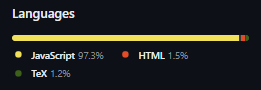
\includegraphics[width=6cm, keepaspectratio]{img/lenguajes.png}
  \caption{Porcentaje de lenguajes usados.}
  \label{fig:lenguajes}
\end{figure}


\section{Importaciones de Bibliotecas JavaScript} 
\label{sec:importaciones}

\begin{itemize}
  \item THREE.js: Biblioteca JavaScript de código abierto para crear y renderizar gráficos en 3D en el navegador web.
  
  \item VRButton.js: Módulo de Three.js que facilita la integración de botones para activar la funcionalidad de realidad virtual (VR) en aplicaciones web.
  
  \item XRControllerModelFactory.js: Módulo de Three.js que proporciona una fábrica para crear modelos de controladores de realidad extendida (XR) para 
  su uso en aplicaciones de realidad virtual y aumentada.

  \item Stats.js: Módulo de Three.js que ofrece una utilidad para monitorear el rendimiento (FPS, uso de memoria) de aplicaciones web 3D en tiempo real.
  
  \item OrbitControls.js: Módulo de Three.js que proporciona controles de órbita para permitir al usuario rotar, acercar y alejar la cámara en una escena 3D de manera interactiva.
  
\end{itemize}


\section{Herramientas de Desarrollo} 
\label{sec:herramientas}

\begin{itemize}
  \item FireFox: Navegador web de código abierto conocido por su enfoque en la privacidad y la personalización.
  
  \item VisualStudioCode: Editor de código fuente de Microsoft altamente personalizable y de código abierto, conocido 
  por su rendimiento y amplia gama de extensiones.
  
  \item GitHub: Plataforma de desarrollo colaborativo de software basada en la nube, que permite a los desarrolladores alojar, revisar, 
  colaborar y desplegar proyectos de software, incluidas aplicaciones web, de manera eficiente y transparente.

  \item Oculus Quest 2: Gafas de realidad virtual autónomas producidas por Oculus (una subsidiaria de Facebook), conocidas 
  por su alta calidad y facilidad de uso. Estas gafas fueron proporcionadas por la universidad para el desarrollo del proyecto.
  
  \item Web XR API Emulator: Herramienta de desarrollo que permite probar y depurar experiencias de realidad virtual y aumentada 
  basadas en WebXR directamente en el navegador web. 
  
\end{itemize}


%%%%%%%%%%%%%%%%%%%%%%%%%%%%%%%%%%%%%%%%%%%%%%%%%%%%%%%%%%%%%%%%%%%%%%%%%%%%%%%%
%%%%%%%%%%%%%%%%%%%%%%%%%%%%%%%%%%%%%%%%%%%%%%%%%%%%%%%%%%%%%%%%%%%%%%%%%%%%%%%%
% DISEÑO E IMPLEMENTACIÓN %
%%%%%%%%%%%%%%%%%%%%%%%%%%%%%%%%%%%%%%%%%%%%%%%%%%%%%%%%%%%%%%%%%%%%%%%%%%%%%%%%

\cleardoublepage
\chapter{Diseño e implementación}
\label{sec:diseno}

En este capítulo, se detalla el desarrollo del proyecto, incluyendo su estructura, los componentes en el entorno 
inmersivo, su funcionamiento, y las interacciones implementadas.


\section{Arquitectura general} 
\label{sec:arquitectura}

El proyecto se estructura en cinco componentes enlazados entre si, representados en la figura~\ref{fig:arquitectura}. Estos componentes serán explicados a continuación:

\begin{itemize}
  \item index.html: Representamos la estructura básica de una página web para una experiencia de realidad virtual (VR). 
  Se define un documento HTML con metadatos y referencias a archivos externos, incluyendo la biblioteca Three.js para gráficos 3D. 
  
  Además, se importa un módulo de JavaScript que inicializa la aplicación VR, creando una instancia de la clase "App" y asignándola a la ventana del navegador. 
  
  Este archivo proporciona una base para el desarrollo de aplicaciones de realidad virtual en la web.
  
  \item app.js: Este script es una aplicación que utiliza la biblioteca Three.js para crear una escena 3D interactiva. Que realiza:
    
    \begin{enumerate}
      \item Importa las bibliotecas necesarias de Three.js para crear la escena.
      \item Carga varias texturas de imágenes para aplicarlas a los materiales de los objetos en la escena.
      \item Define algunas variables y objetos necesarios para el funcionamiento de la aplicación.
      \item Crea una clase App que inicializa la escena, la cámara, la iluminación y los controles.
      \item Dentro de la clase App, hay métodos para manejar el control de los dispositivos de entrada de VR, como los controladores y sus eventos.
      \item Contiene un método para construir los modelos de los controladores de VR.
      \item Otro método se encarga de manejar la lógica de la animación y la interacción del usuario con la escena.
      \item Y finalmente, tenemos un método de renderizado que se ejecuta en bucle y actualiza la escena en cada fotograma.
    \end{enumerate}

  \item imágenes: En la arquitectura del proyecto, tenemos una carpeta llamada "imagenes" que contiene todas las imágenes utilizadas en la aplicación. 
  Dentro de esta carpeta, tenemos subcarpetas para organizar las imágenes de acuerdo con su propósito.

  Cada imagen se carga en la aplicación utilizando el constructor THREE.TextureLoader().load(), 
  proporcionando la ruta relativa desde el punto donde se está ejecutando el código hacia la ubicación de la imagen en la estructura de carpetas.

  \item sceneObjets: Este archivo es un módulo de funciones que proporciona diferentes objetos tridimensionales (3D) utilizando la biblioteca Three.js. 
  Cada función devuelve un objeto con geometría y material específicos.

  \begin{enumerate}
    \item Sphere: Devuelve una esfera roja con una geometría esférica y un material básico.
    \item Side: Devuelve un objeto rectangular con una textura proporcionada, usado como pared en la escena.
    \item Box: Devuelve una caja con una textura proporcionada, usado como UA y Proxy en la escena.
    \item Wall: Devuelve un plano grande con una textura proporcionada, usado como pantalla en la escena.
    \item Logo: Devuelve un plano con una textura proporcionada, representando logotipo.
    \item Floor: Devuelve un plano grande con una textura proporcionada, usado para el suelo de la escena.
  \end{enumerate}

  Cada función utiliza diferentes geometrías y materiales para crear los objetos 3D. 
  También configura propiedades específicas de los materiales, como envoltura de textura y repetición.
  
  \item jsm: Esta carpeta contiene módulos JavaScript utilizados en el proyecto. Estos módulos son archivos independientes que proporcionan funcionalidades específicas para la aplicación. 
  Aquí está la estructura de la carpeta:

  \begin{enumerate}
    \item build: En esta subcarpeta se encuentran los archivos de construcción de la biblioteca Three.js, 
    que proporcionan la funcionalidad principal de renderización en 3D. El archivo principal utilizado es three.module.js, 
    que importa todas las funcionalidades esenciales de Three.js.
    \item webxr: Aquí están los módulos relacionados con WebXR, una API que permite crear experiencias de realidad virtual (VR) y realidad aumentada (AR) en el navegador. 
    Por ejemplo, VRButton.js proporciona un botón para activar la experiencia de realidad virtual, mientras que XRControllerModelFactory.js 
    permite crear modelos visuales para los controladores de VR.
    \item libs: Esta subcarpeta contiene bibliotecas adicionales utilizadas en el proyecto. 
    En particular, stats.module.js proporciona una herramienta para medir el rendimiento de la aplicación 
    mediante la visualización de estadísticas, como el número de fotogramas por segundo.
    \item controls: Aquí están los módulos relacionados con el control de la cámara y la escena en la aplicación. 
    Por ejemplo, OrbitControls.js proporciona controles para permitir al usuario mover y rotar la cámara 
    alrededor de la escena, lo que facilita la navegación en entornos 3D.
  \end{enumerate}

  Por lo tanto, la carpeta 'jsm' organiza los módulos JavaScript utilizados en el proyecto, 
  proporcionando funcionalidades esenciales, soporte para WebXR, herramientas de medición de rendimiento y controles de cámara. 
  Estos módulos se importan en la aplicación según sea necesario para agregar las características deseadas.

\end{itemize}

\begin{figure}
  \centering
  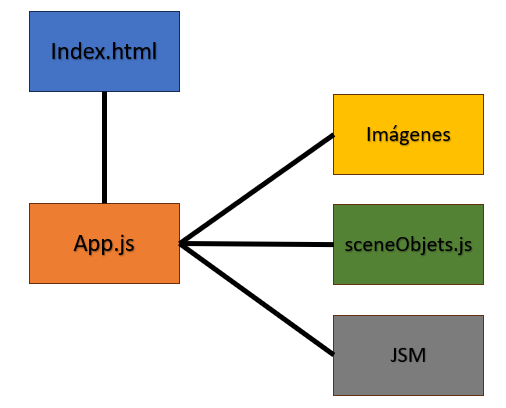
\includegraphics[width=9cm, keepaspectratio]{img/estructura.png}
  \caption{Estructura del proyecto}
  \label{fig:arquitectura}
\end{figure}


\section{Escena} 
\label{sec:escena}

La escena virtual implementada se desarrolla utilizando la biblioteca Three.js, 
que permite la creación de gráficos 3D en un entorno web. Este proyecto configura un entorno interactivo 
que simula un sistema de comunicación, donde se pueden visualizar los intercambios de mensajes entre diferentes usuarios y un proxy.

\textbf{Estructura Básica}

\begin{itemize}
  \item \textbf{Cámara y Controles:} La cámara se configura con una perspectiva que permite al usuario tener una vista adecuada del entorno virtual. 
  Se utiliza OrbitControls para permitir al usuario interactuar con la vista, rotando y acercando/alejando la escena.
  
  \item \textbf{Iluminación:} Se añade iluminación hemisférica para simular una luz suave y direccional 
  para destacar objetos específicos dentro de la escena.

  \item \textbf{Renderizado:} Se establece un renderizado con antialiasing para mejorar la calidad visual de los bordes de los objetos en la escena.
  
\end{itemize}

\textbf{Objetos en la Escena}

\begin{itemize}
  \item \textbf{Suelo y Paredes:} Se utilizan texturas cargadas para crear un suelo y paredes que encierran la escena, proporcionando un fondo estático.
  
  \item \textbf{Objetos Interactivos:} Se crean varias cajas y esferas que representan a diferentes usuarios (UA1, UA2) y un proxy. 
  Estos objetos se pueden interactuar mediante eventos controlados por los controladores de realidad virtual.

  \item \textbf{Indicadores Visuales:} Se utilizan logos y texturas para indicar estados como "start" y "stop", mostrando visualmente el flujo de la simulación.
  
\end{itemize}

\textbf{Interacción y Dinámica}

\begin{itemize}
  \item \textbf{Inicio de Eventos:} La interacción comienza cuando el usuario activa controles específicos en los controladores de realidad virtual. 
  Esto puede alterar el estado de los objetos (por ejemplo, cambiar el color para indicar actividad) y cambiar texturas que 
  representan diferentes mensajes enviados y recibidos en la comunicación.
  
  \item \textbf{Simulación de Mensajes:} Los objetos esféricos se mueven entre las cajas para simular el envío de mensajes. 
  La ruta y la dirección de estos objetos dependen de las interacciones del usuario y el flujo del protocolo simulado.

  \item \textbf{Animación de Paquetes RTP:} En ciertos puntos, esferas adicionales se mueven para simular la transmisión de paquetes RTP, 
  indicando el intercambio de media en una llamada establecida.
  
\end{itemize}


\textbf{Implementación Técnica}

\begin{itemize}
  \item \textbf{Controladores XR:} Se configuran controladores para manejar la interacción en un entorno de realidad extendida (XR). 
  Esto incluye la gestión de eventos de selección y conexión de dispositivos.
  
  \item \textbf{Animación y Actualización de la Escena:} Los objetos esféricos se mueven entre las cajas para simular el envío de mensajes. 
  La ruta y la dirección de estos objetos dependen de las interacciones del usuario y el flujo del protocolo simulado.

  \item \textbf{Animación de Paquetes RTP:} La lógica para mover objetos y actualizar estados se ejecuta dentro de un bucle 
  de animación que recalcula posiciones y estados basados en la interacción del usuario.
  
\end{itemize}

\begin{figure}
  \centering
  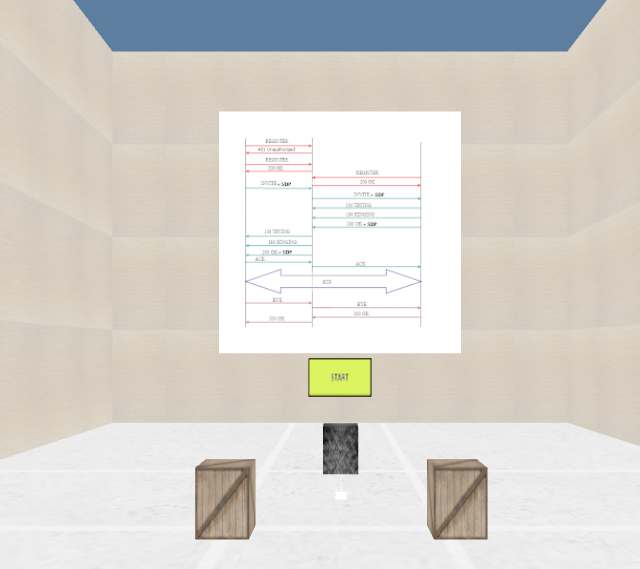
\includegraphics[width=9cm, keepaspectratio]{img/escena.png}
  \caption{Escena del proyecto}
  \label{fig:arquitectura}
\end{figure}


\section{Controles de Realidad Virtual}
\label{sec:controles_vr}

La implementación de controles de realidad virtual en la aplicación proporciona una interfaz interactiva que mejora significativamente la experiencia del usuario, 
permitiendo una manipulación intuitiva y directa de la escena virtual.

\subsection{Configuración de los Controladores VR}
\label{subsec:configuracion_controladores_vr}

Los controladores VR son dispositivos físicos que los usuarios sostienen en sus manos y que detectan sus movimientos y gestos en el espacio tridimensional. 
Estos están equipados con una variedad de sensores y botones que permiten una gama amplia de interacciones:

\begin{itemize}
  \item \textbf{Botones y Gatillos}: Utilizados para realizar selecciones y activar eventos dentro de la aplicación. 
  Por ejemplo, un usuario puede iniciar la transmisión de mensajes al presionar el botón "Start".
  \item \textbf{Sensores de Movimiento}: Capturan el posicionamiento y la orientación de las manos del usuario, 
  permitiendo manipular objetos o navegar por la escena con movimientos naturales.
\end{itemize}

\begin{figure}
  \centering
  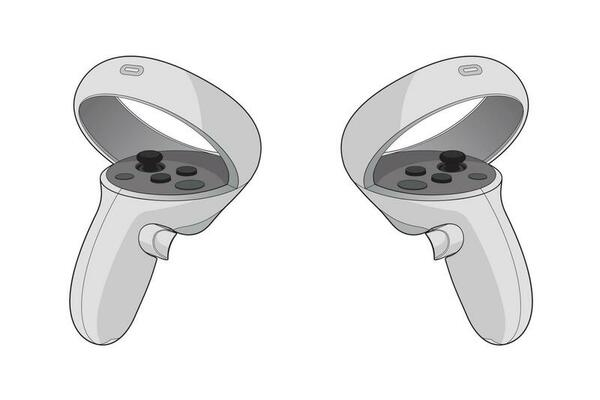
\includegraphics[width=6cm, keepaspectratio]{img/controlador.png}
  \caption{Controlador VR}
  \label{fig:controlador}
\end{figure}


\subsection{Interacción Mediante Controladores VR}
\label{subsec:interaccion_controladores_vr}

La interacción con la escena se realiza a través de los controladores VR de la siguiente manera:

\begin{itemize}
  \item \textbf{Selección y Manipulación}: Los usuarios apuntan a objetos virtuales con los controladores y utilizan 
  botones para seleccionarlos. Esto puede incluye activar elementos dentro de la escena.
  \item \textbf{Navegación}: Mediante el uso del gatillo en los controladores, 
  los usuarios pueden desplazarse por la escena virtual, acercándose o alejándose de los objetos o desplazándose lateralmente.
  \item \textbf{Interacción Contextual}: La aplicación cambia la funcionalidad de la escena 
  basándose el estado del objeto con el que el usuario está interactuando, 
  cambiando modos de visualización o ajustando parámetros específicos de los objetos.
\end{itemize}

\subsection{Implementación Técnica}
\label{subsec:implementacion_tecnica_vr}

La implementación técnica de los controladores VR en la aplicación utiliza la API de WebXR, integrada con Three.js, para gestionar la entrada 
de los dispositivos de realidad virtual. El código configura cada controlador para responder a eventos como `selectstart` y `selectend`, 
lo que permite detectar interacciones como pulsaciones de botones y liberaciones. Adicionalmente, se emplean rayos virtuales (`raycasting`) 
para determinar qué objetos están siendo apuntados por los controladores, facilitando así una interacción precisa.


En la implementación de la aplicación, hacemos un uso específico de los botones trigger de los controladores VR para facilitar una interacción 
intuitiva y efectiva dentro del entorno virtual. Cada trigger tiene un propósito bien definido que mejora la experiencia del 
usuario y la funcionalidad de la aplicación:

\begin{itemize}
  \item \textbf{Trigger del Controlador Izquierdo}: Este botón se utiliza para la navegación dentro de la escena. Al presionar el trigger del controlador izquierdo, 
  el usuario puede desplazarse hacia donde esté mirando con las gafas de realidad virtual, lo que permite una navegación intuitiva y natural. 
  Esta funcionalidad es fundamental para explorar diferentes áreas de la escena de manera fluida.
  
  \item \textbf{Trigger del Controlador Derecho}: El trigger del controlador derecho está configurado para interactuar con objetos 
  específicos de la escena. Cuando se presiona este botón, se puede seleccionar o activar elementos dentro de la escena, 
  como iniciar una simulación, modificar parámetros de un objeto, o ejecutar acciones específicas relacionadas con los objetos con los que se interactúa. 
  Esta interacción es esencial para manipular elementos de la aplicación y para participar activamente en las simulaciones y demostraciones que se presentan en el entorno virtual.
\end{itemize}

La programación de estos triggers se realiza a través del manejo de eventos en JavaScript, utilizando la API de WebXR para detectar y responder 
a las acciones del usuario. Este diseño permite un control preciso sobre la aplicación, ofreciendo a los usuarios una manera clara y directa 
de interactuar con la interfaz y con los elementos virtuales de la escena.

\begin{figure}
  \centering
  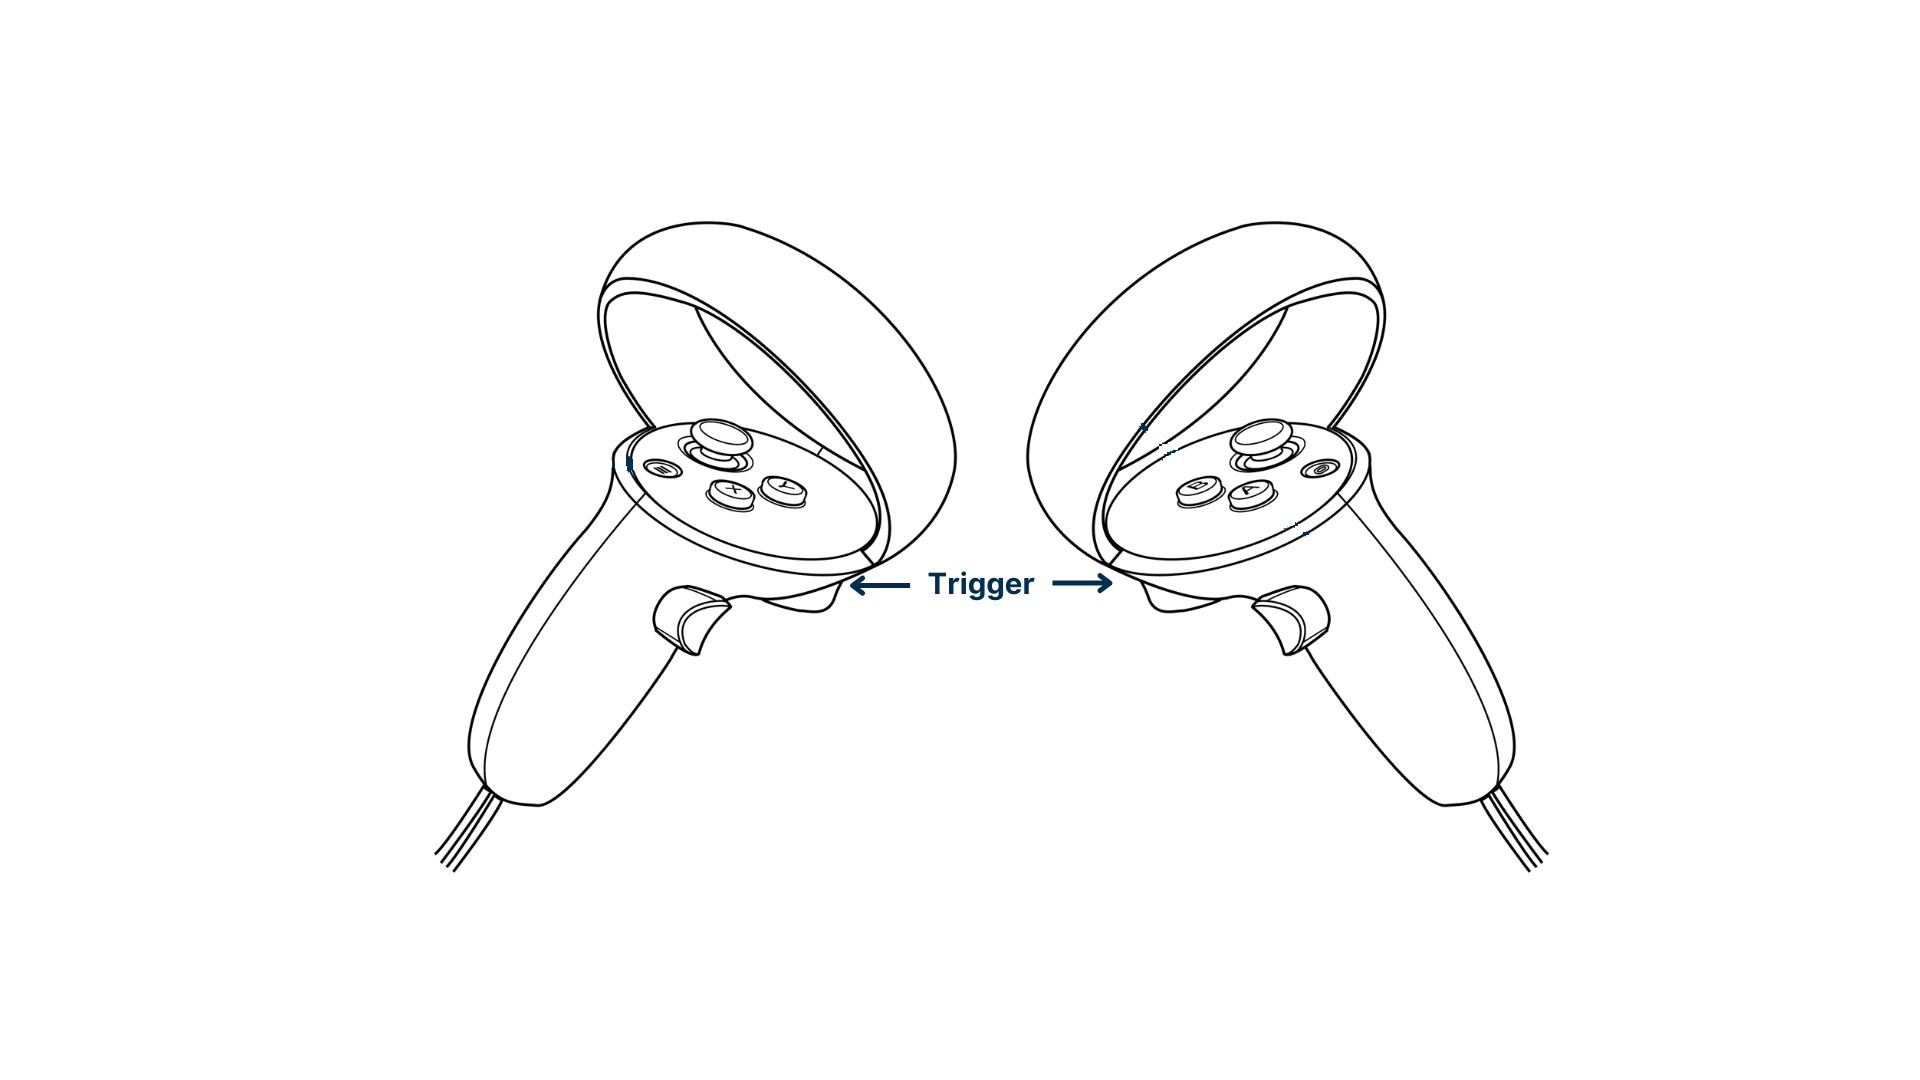
\includegraphics[width=6cm, keepaspectratio]{img/BotonesControlador.png}
  \caption{Botones controlador VR}
  \label{fig:controladorBotones}
\end{figure}

%%%%%%%%%%%%%%%%%%%%%%%%%%%%%%%%%%%%%%%%%%%%%%%%%%%%%%%%%%%%%%%%%%%%%%%%%%%%%%%%
%%%%%%%%%%%%%%%%%%%%%%%%%%%%%%%%%%%%%%%%%%%%%%%%%%%%%%%%%%%%%%%%%%%%%%%%%%%%%%%%
% EXPERIMENTOS Y VALIDACIÓN %
%%%%%%%%%%%%%%%%%%%%%%%%%%%%%%%%%%%%%%%%%%%%%%%%%%%%%%%%%%%%%%%%%%%%%%%%%%%%%%%%

\cleardoublepage
\chapter{Experimentos y validación}
\label{chap:experimentos}

Este capítulo se introdujo como requisito en 2019. 
Describe los experimentos y casos de test que tuviste que implementar para validar tus resultados. 
Incluye también los resultados de validación que permiten afirmar que tus resultados son correctos. 


%%%%%%%%%%%%%%%%%%%%%%%%%%%%%%%%%%%%%%%%%%%%%%%%%%%%%%%%%%%%%%%%%%%%%%%%%%%%%%%%
%%%%%%%%%%%%%%%%%%%%%%%%%%%%%%%%%%%%%%%%%%%%%%%%%%%%%%%%%%%%%%%%%%%%%%%%%%%%%%%%
% RESULTADOS %
%%%%%%%%%%%%%%%%%%%%%%%%%%%%%%%%%%%%%%%%%%%%%%%%%%%%%%%%%%%%%%%%%%%%%%%%%%%%%%%%

\cleardoublepage
\chapter{Resultados}
\label{chap:resultados}

En este capítulo, se presentan los resultados derivados de las interacciones con los objetos de la escena en la aplicación 
de realidad virtual desarrollada. Se describirá cómo distintas selecciones de objetos generan resultados visuales y 
funcionales diferentes, lo que demuestra la dinámica y la reactividad de la aplicación ante las acciones del usuario.

\section{Descripción de las Interacciones}
\label{sec:descripcion_interacciones}
Las interacciones en la aplicación permiten a los usuarios seleccionar objetos virtuales, 
los cuales alteran el estado de la escena y desencadenan eventos específicos. 

Como se mencionó en la Sección 4.3.3, para lograr estos resultados es necesario utilizar controladores VR. 
Estos dispositivos permiten a los usuarios moverse por la escena e interactuar con los objetos de manera intuitiva y efectiva.
La selección se realiza apuntando hacia el objeto con el controlador derecho y activando el trigger.

Cada objeto tiene asociadas consecuencias específicas que se detallan a continuación:

\subsection{Interacción con UA1}
\label{subsec:objeto_ua1}

Este objeto representa un usuario dentro del entorno virtual y está visualizado como una caja 
de madera ubicada en la parte izquierda de la escena.

Al interactuar con UA1, este cambiará de color y podrán obtener dos posibles resultados, los cuales dependen 
de si el intercambio de paquetes ha sido inicializado o no.

\subsubsection{Intercambio de paquetes no iniciado}
\label{subsubsec:Intercambio_NoIniciado}
Si el intercambio de paquetes no ha sido inicializado, en la pantalla situada en la pared central se mostrarán 
los atributos del usuario en estado vacío, indicando los valores que deberían ser completados, mostrados en la figura~\ref{fig:UA1_NoIniciado}. 
Esta visualización es esencial para comprender los requisitos iniciales de configuración del usuario en la red. Estos tributos son:

\begin{itemize}
  \item \textbf{'account'}: ['username', 'passwd']
  \item \textbf{'uaserver'}: ['ip', 'puerto']
  \item \textbf{'rtpaudio'}: ['puerto']
  \item \textbf{'regproxy'}: ['ip', 'puerto']
  \item \textbf{'log'}: ['path']
  \item \textbf{'audio'}: ['path']
\end{itemize}

\begin{figure}
  \centering
  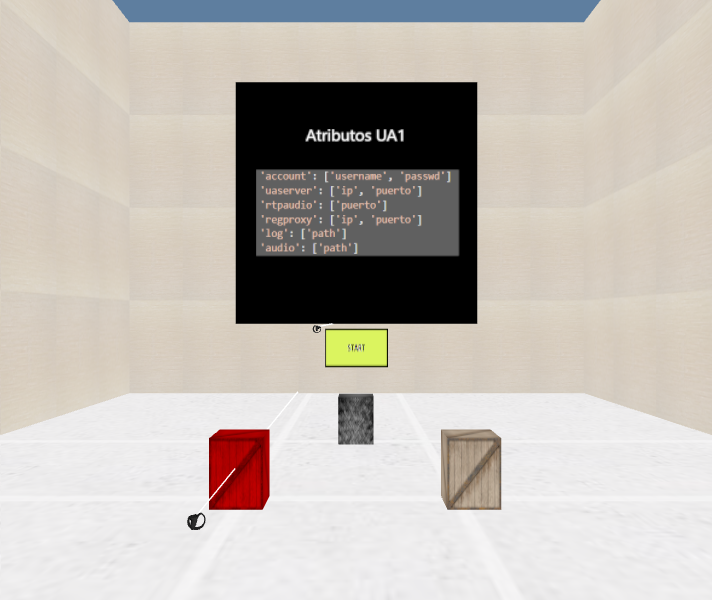
\includegraphics[width=15cm, keepaspectratio]{img/resultados/UA1_NoIniciado.png}
  \caption{Estado inicial del UA1}
  \label{fig:UA1_NoIniciado}
\end{figure}


\subsubsection{Intercambio de paquetes iniciado}
\label{subsubsec:Intercambio_Iniciado}
Una vez que el intercambio de paquetes ha sido iniciado, en la misma pantalla se 
actualizarán los atributos del usuario con valores específicos y correctos para su funcionamiento mostrados en la figura~\ref{fig:UA1_Iniciado}.  
Este cambio refleja cómo el sistema procesa y responde a las interacciones, ofreciendo un feedback visual del estado operativo del usuario.

\begin{figure}
  \centering
  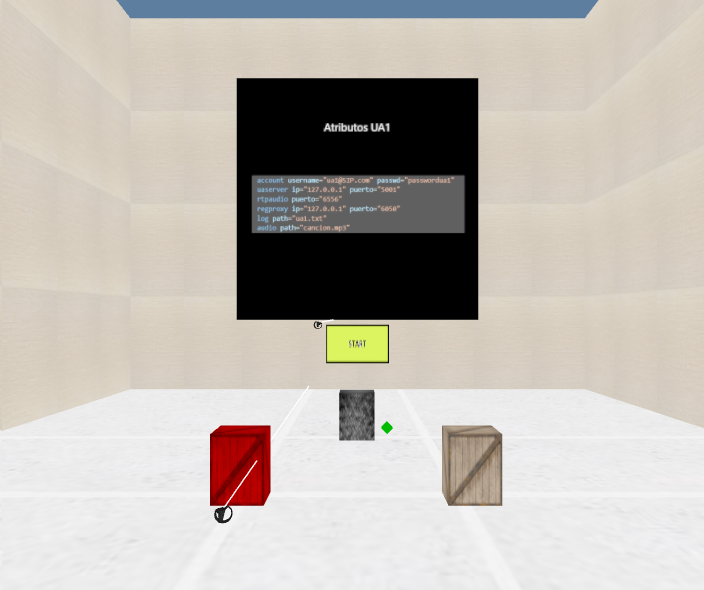
\includegraphics[width=15cm, keepaspectratio]{img/resultados/UA1_Iniciado.png}
  \caption{Atributos UA1 con valores específicos}
  \label{fig:UA1_Iniciado}
\end{figure}


\subsection{Interacción con el Proxy}
\label{subsec:objeto_proxy}

Este objeto representa un servidor proxy en el entorno virtual y está visualizado como una caja con textura oscura,
ubicada en la parte central de la escena.

Al interactuar con el Proxy, este cambiará de color y dependiendo del estado de la interacción con los usuarios (UA1 y UA2), 
se pueden obtener diferentes resultados, influenciados por si el intercambio de paquetes ha sido iniciado o no.

\subsubsection{Intercambio de paquetes no iniciado}
\label{subsubsec:Proxy_Intercambio_NoIniciado}
Si el intercambio de paquetes no ha sido inicializado, la interacción con el Proxy mostrará en la pantalla sus atributos 
con la información que deben ser completados, donde no se procesan aún los paquetes, mostrados en la figura~\ref{fig:Proxy_NoIniciado}. Estos campos son:

\begin{itemize}
  \item \textbf{'server'}: ['name', 'ip', 'puerto']
  \item \textbf{'database'}: ['path', 'passwdpath']
  \item \textbf{'log'}: ['path']
\end{itemize}

\begin{figure}
  \centering
  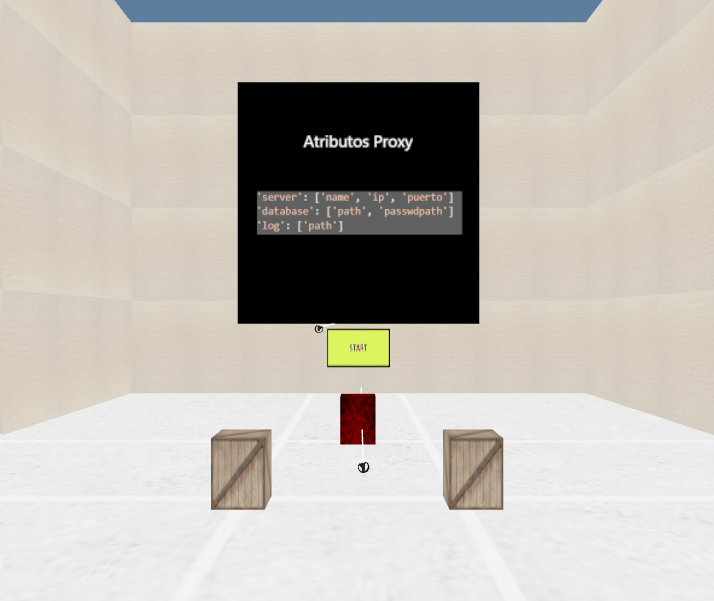
\includegraphics[width=15cm, keepaspectratio]{img/resultados/Proxy_NoIniciado.png}
  \caption{Estado inicial del Proxy}
  \label{fig:Proxy_NoIniciado}
\end{figure}

\subsubsection{Intercambio de paquetes iniciado}
\label{subsubsec:Proxy_Intercambio_Iniciado}
Una vez que el intercambio de paquetes ha sido iniciado, el Proxy procesará y dirigirá los paquetes entre los usuarios correspondientes, 
reflejando este flujo en la interfaz con actualizaciones dinámicas. Al seleccionar el Proxy se mostrarán sus atributos con valores específicos 
y correctos para su funcionamiento, mostrados en la figura~\ref{fig:Proxy_Iniciado}.

\begin{figure}
  \centering
  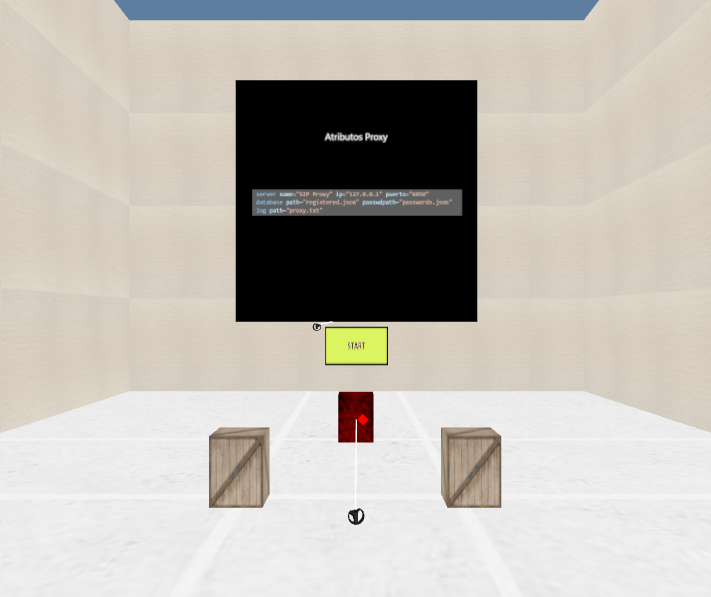
\includegraphics[width=15cm, keepaspectratio]{img/resultados/Proxy_Iniciado.png}
  \caption{Atributos Proxy con valores específicos}
  \label{fig:Proxy_Iniciado}
\end{figure}


\subsection{Interacción con UA2}
\label{subsec:objeto_ua1}

Este objeto representa un usuario dentro del entorno virtual y está visualizado como una caja 
de madera ubicada en la parte derecha de la escena.

Al interactuar con UA2, este cambiará de color y podrán obtener dos posibles resultados, los cuales dependen 
de si el intercambio de paquetes ha sido inicializado o no.

\subsubsection{Intercambio de paquetes no iniciado}
\label{subsubsec:Intercambio_NoIniciado}
Si el intercambio de paquetes no ha sido inicializado, en la pantalla situada en la pared central se mostrarán 
los atributos del usuario en estado vacío, indicando los valores que deberían ser completados, mostrados en la figura~\ref{fig:UA2_NoIniciado}. 
Esta visualización es esencial para comprender los requisitos iniciales de configuración del usuario en la red. Estos tributos son:

\begin{itemize}
  \item \textbf{'account'}: ['username', 'passwd']
  \item \textbf{'uaserver'}: ['ip', 'puerto']
  \item \textbf{'rtpaudio'}: ['puerto']
  \item \textbf{'regproxy'}: ['ip', 'puerto']
  \item \textbf{'log'}: ['path']
  \item \textbf{'audio'}: ['path']
\end{itemize}

\begin{figure}
  \centering
  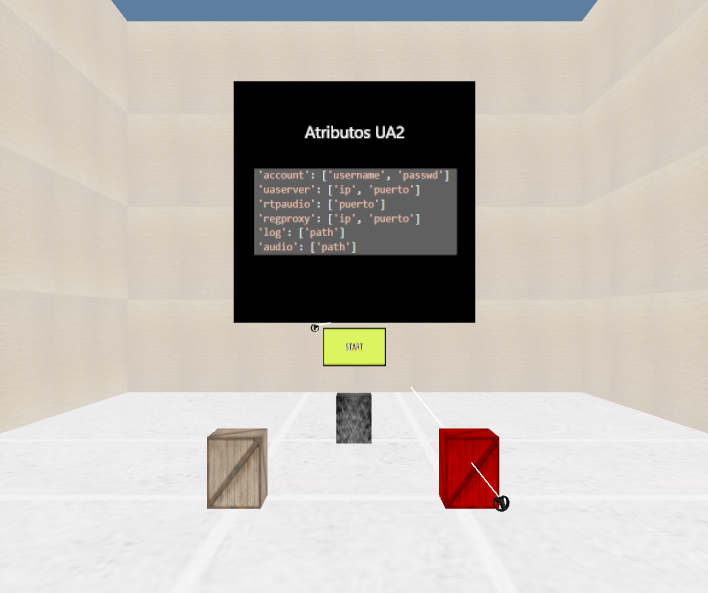
\includegraphics[width=15cm, keepaspectratio]{img/resultados/UA2_NoIniciado.png}
  \caption{Estado inicial del UA2}
  \label{fig:UA2_NoIniciado}
\end{figure}


\subsubsection{Intercambio de paquetes iniciado}
\label{subsubsec:Intercambio_Iniciado}
Una vez que el intercambio de paquetes ha sido iniciado, en la misma pantalla se 
actualizarán los atributos del usuario con valores específicos y correctos para su funcionamiento mostrados en la figura~\ref{fig:UA2_Iniciado}.  
Este cambio refleja cómo el sistema procesa y responde a las interacciones, ofreciendo un feedback visual del estado operativo del usuario.

\begin{figure}
  \centering
  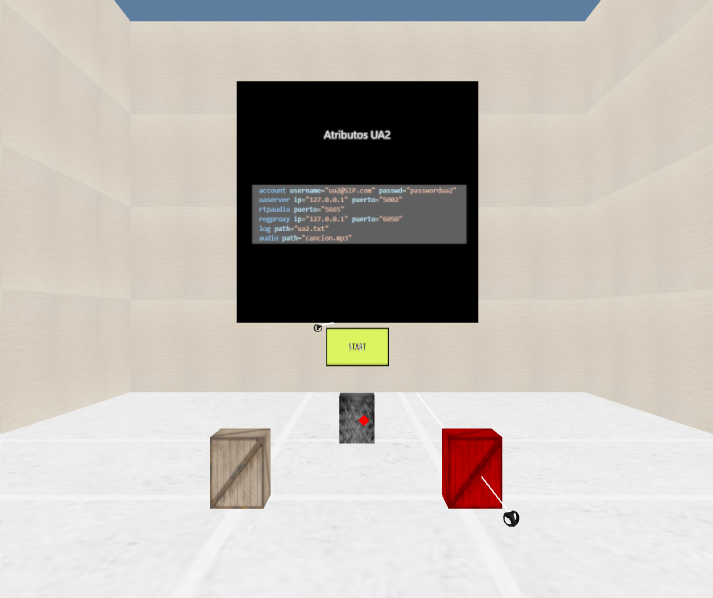
\includegraphics[width=15cm, keepaspectratio]{img/resultados/UA2_Iniciado.png}
  \caption{Atributos UA2 con valores específicos}
  \label{fig:UA2_Iniciado}
\end{figure}


\subsection{Interacción con paquetes}
\label{subsec:objeto_paquetes}
En el entorno de realidad virtual, los paquetes se representan en forma de esferas que simulan la transmisión de datos en una red. 
Estas esferas visualizan claramente el flujo de información, con un origen, un destino y un color claramente definidos, 
dependiendo del tipo de intercambio en el que participan.

Al seleccionar uno de estos paquetes, el sistema mostrará información detallada contenida en el paquete, 
incluyendo una representación visual del flujo de transmisión que indica su origen, destino y la dirección del flujo.

El proceso y secuencia de intercambio de paquetes en este proyecto se ilustra en la siguiente figura~\ref{fig:Secuencia_Paquetes}, donde se puede observar el orden 
específico seguido durante las simulaciones.

Esta figura~\ref{fig:Secuencia_Paquetes} ilustra un intercambio de mensajes de protocolo típico en una comunicación de red utilizando el Protocolo de Inicio de Sesión (SIP). 
Este diagrama de flujo representa la secuencia de mensajes entre dos usuarios que intentan establecer una comunicación, 
pasando por un proceso de registro y luego de llamada.

\begin{figure}
  \centering
  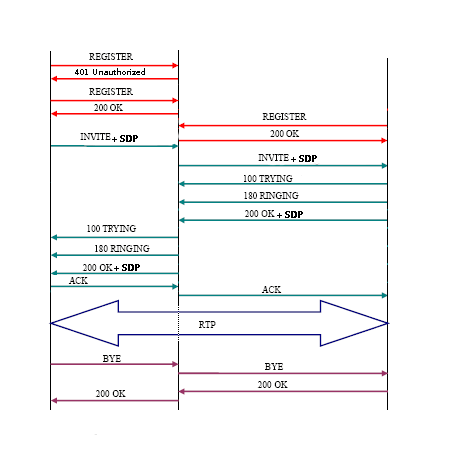
\includegraphics[width=18cm, keepaspectratio]{img/resultados/Secuencia_Paquetes.png}
  \caption{Secuencia del intercambio de paquetes}
  \label{fig:Secuencia_Paquetes}
\end{figure}

\subsubsection{Desglose de la Secuencia de Comunicación}
\label{subsubsec:secuencia_comunicación}

Inicialmente, el proceso comienza con un intento de registro, donde el usuario A (UA1) envía un mensaje "REGISTER" al servidor, 
representado en la figura~\ref{fig:01-Register_UA1}. 
Si no está autorizado, recibe un "401 Unauthorized", mostrado en la figura~\ref{fig:02-Unauthorized}, 
lo que obliga al usuario (UA1) a realizar otro intento de "REGISTER", el cual, es aceptado,
y se confirma con una respuesta "200 OK", ilustrado en la figura~\ref{fig:02-200OK}, 
indicando que el registro se ha completado con éxito.

A continuación, se registra el usuario B (UA2) enviando un mensaje "REGISTER" al servidor,
representado en la figura~\ref{fig:03-Register_UA2}. 
Siendo este aceptado y confirmado con una respuesta de "200 OK", ilustrado en la figura~\ref{fig:04-200OK}.

La fase de llamada comienza con un "INVITE" acompañado de una descripción de la sesión (SDP), escenificado en la figura~\ref{fig:05-Invite}, 
que contiene los detalles para establecer la comunicación. 
Este mensaje es respondido con un "100 TRYING", evidenciado en la figura~\ref{fig:07-Trying},
seguido de un "180 RINGING", ilustrado en la figura~\ref{fig:08-Ringing}, 
que indica que la llamada está siendo procesada y que el otro usuario está siendo alertado de la llamada entrante. 
Cuando el usuario B (UA2) acepta la llamada, envía una respuesta "200 OK + SDP", representado en la figura~\ref{fig:09-200OKSDP}, 
que contiene la confirmación y los detalles necesarios para establecer la comunicación. 
El usuario A (UA1) confirma recibir esta información con un "ACK", mostrado en la figura~\ref{fig:13-ACK}.

Una vez establecida la llamada, los datos multimedia se transmiten a través de 
paquetes "RTP" (Protocolo de Transporte en Tiempo Real), escenificado en la figura~\ref{fig:15-RTP}, 
representados por las esferas azules. Este intercambio continúa hasta que uno de los usuarios decide terminar la llamada, 
enviando un mensaje "BYE", ilustrado en la figura~\ref{fig:16-BYE}. 
El fin de la llamada es confirmado por el otro usuario con un "200 OK", representado en la figura~\ref{fig:18-200OK}, 
cerrando así la sesión de comunicación.
% Bloque 1 %
\begin{figure}
  \centering
  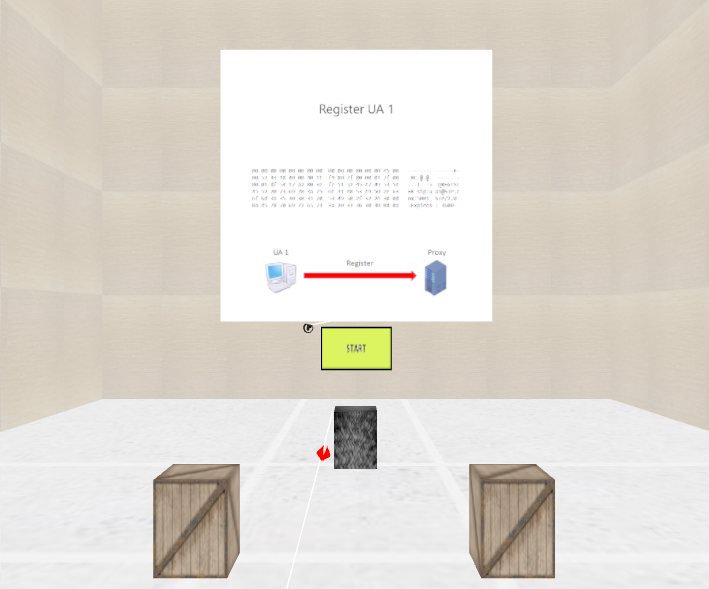
\includegraphics[width=15cm, keepaspectratio]{img/resultados/01-Register_UA1.png}
  \caption{Mensaje de Registro Inicial de UA1}
  \label{fig:01-Register_UA1}
\end{figure}

\begin{figure}
  \centering
  \includegraphics[width=15cm, keepaspectratio]{img/resultados/02-Unauthorized.png}
  \caption{Respuesta 401 Unauthorized a UA1}
  \label{fig:02-Unauthorized}
\end{figure}

\begin{figure}
  \centering
  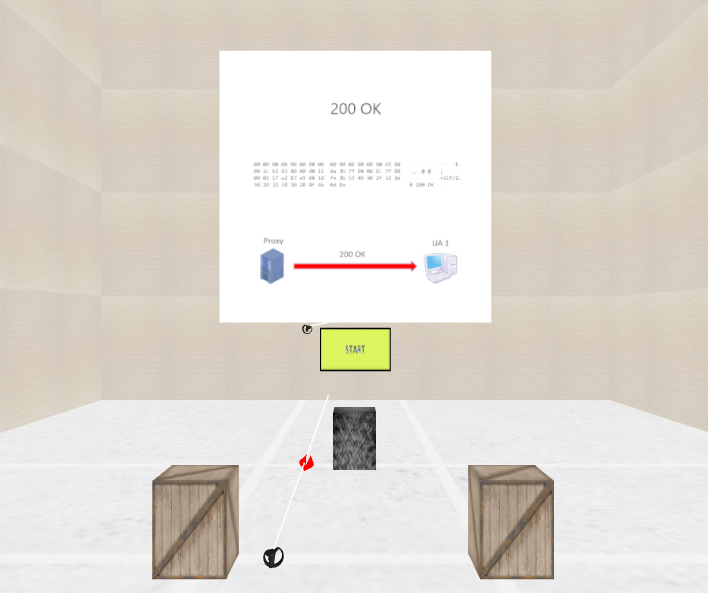
\includegraphics[width=15cm, keepaspectratio]{img/resultados/02-200OK.png}
  \caption{Registro de UA1 Exitoso con 200 OK}
  \label{fig:02-200OK}
\end{figure}
% Bloque 2 %
\begin{figure}
  \centering
  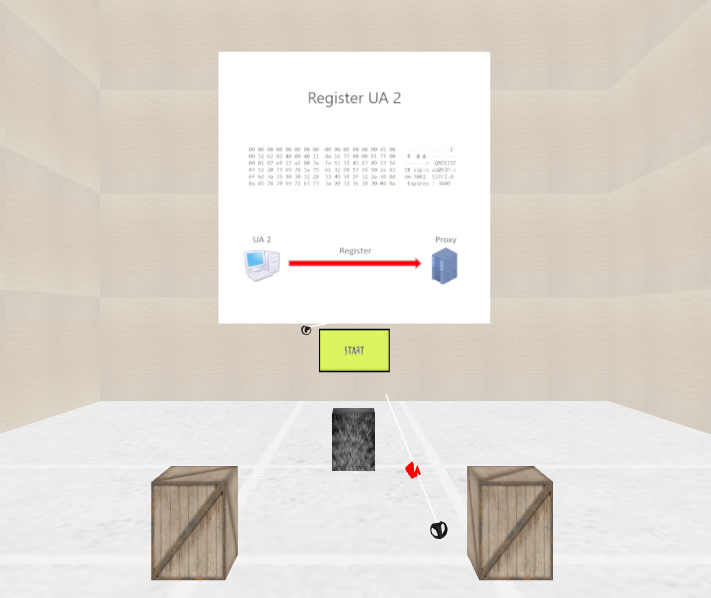
\includegraphics[width=15cm, keepaspectratio]{img/resultados/03-Register_UA2.png}
  \caption{Mensaje de Registro Inicial de UA2}
  \label{fig:03-Register_UA2}
\end{figure}

\begin{figure}
  \centering
  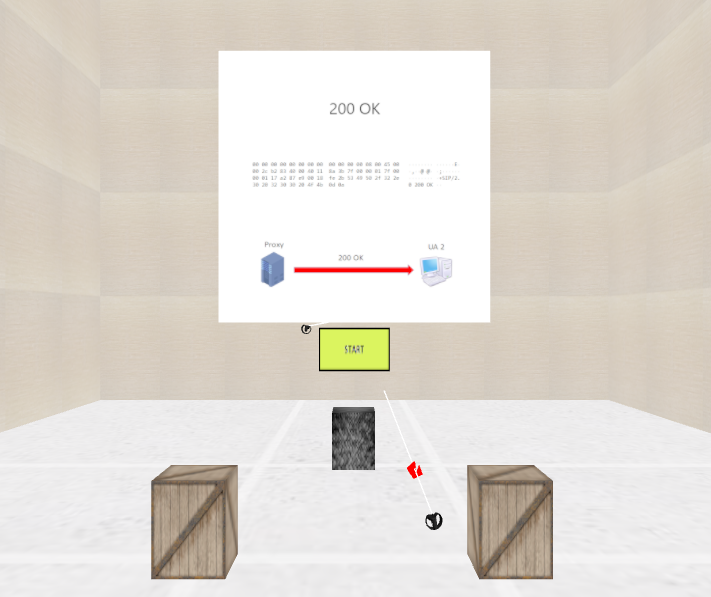
\includegraphics[width=15cm, keepaspectratio]{img/resultados/04-200OK.png}
  \caption{Registro de UA2 Exitoso con 200 OK}
  \label{fig:04-200OK}
\end{figure}

% Bloque 3 %
\begin{figure}
  \centering
  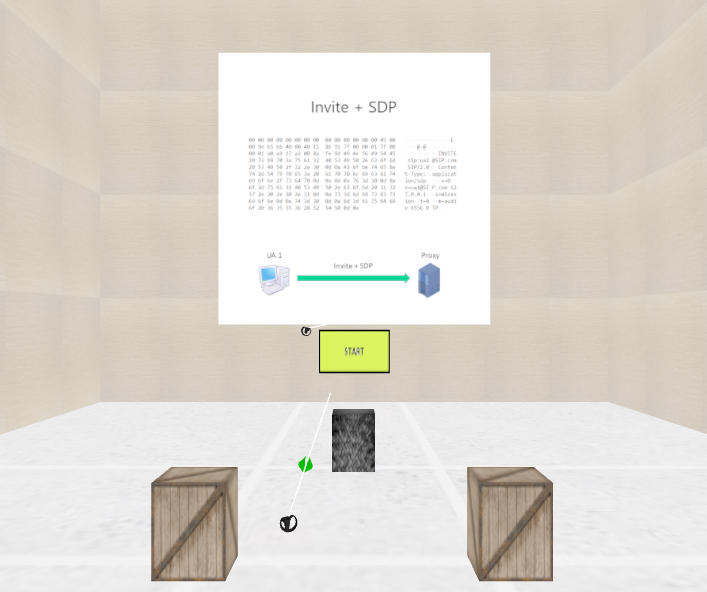
\includegraphics[width=15cm, keepaspectratio]{img/resultados/05-Invite.png}
  \caption{Inicio de Llamada con el Mensaje INVITE de UA1}
  \label{fig:05-Invite}
\end{figure}

\begin{figure}
  \centering
  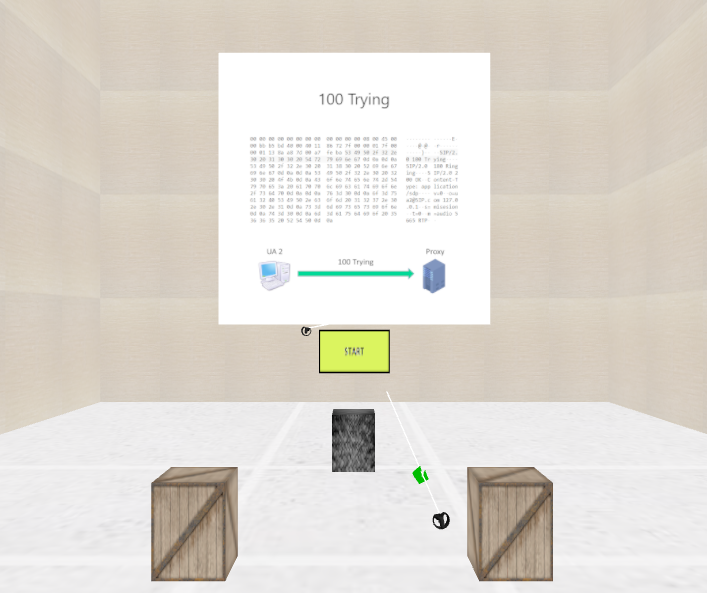
\includegraphics[width=15cm, keepaspectratio]{img/resultados/07-Trying.png}
  \caption{Respuesta TRYING de UA2 Indicando Procesamiento}
  \label{fig:07-Trying}
\end{figure}

\begin{figure}
  \centering
  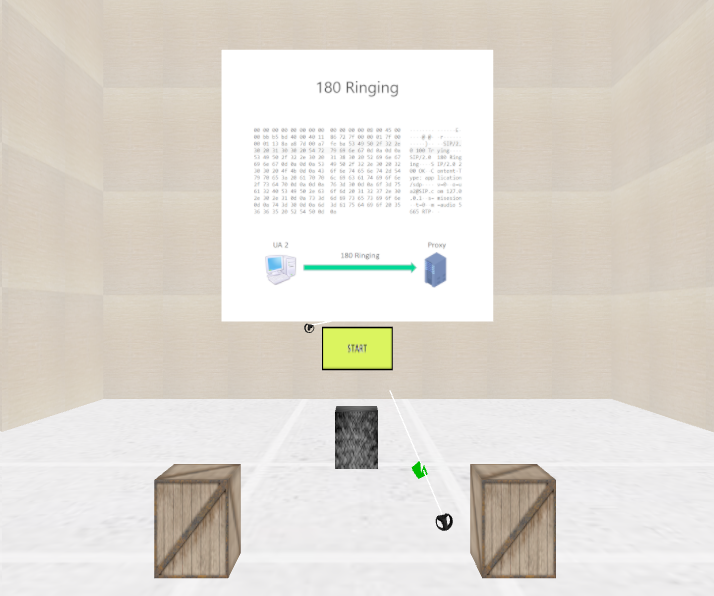
\includegraphics[width=15cm, keepaspectratio]{img/resultados/08-Ringing.png}
  \caption{Alerta de Llamada con el Mensaje RINGING de UA2}
  \label{fig:08-Ringing}
\end{figure}

\begin{figure}
  \centering
  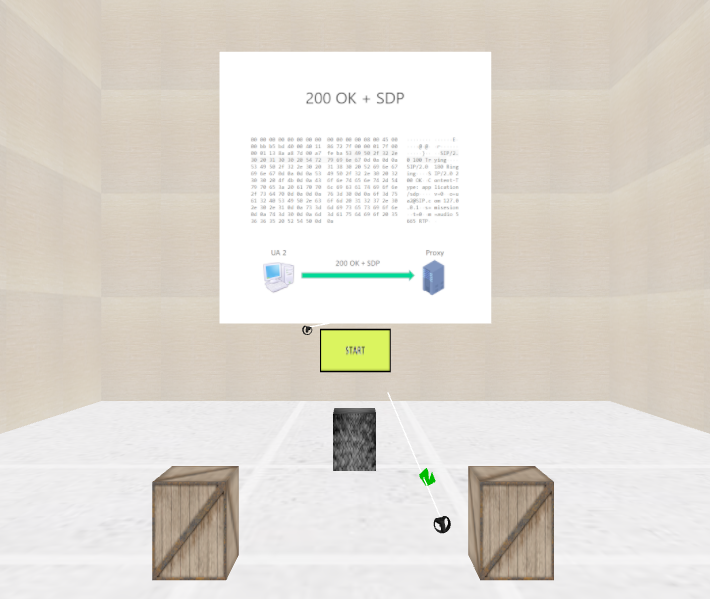
\includegraphics[width=15cm, keepaspectratio]{img/resultados/09-200OKSDP.png}
  \caption{Confirmación de Llamada con 200 OK + SDP de UA2}
  \label{fig:09-200OKSDP}
\end{figure}

\begin{figure}
  \centering
  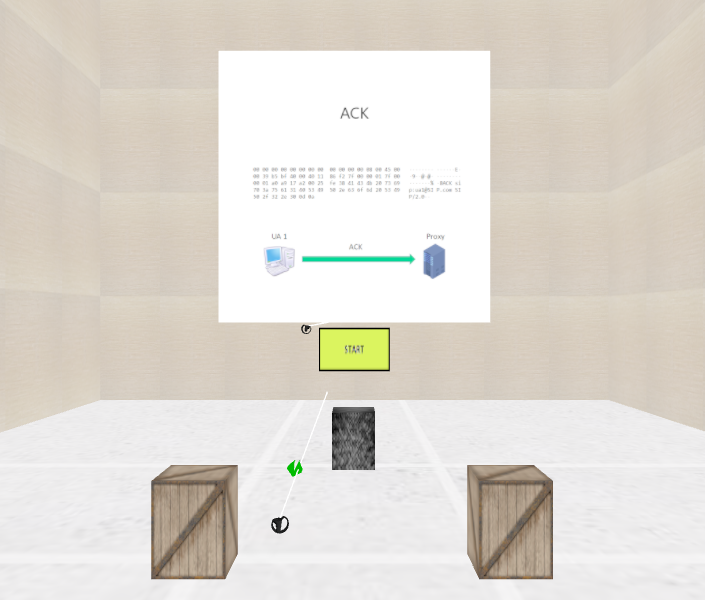
\includegraphics[width=15cm, keepaspectratio]{img/resultados/13-ACK.png}
  \caption{Reconocimiento ACK de UA1 Completando el Establecimiento de la Llamada}
  \label{fig:13-ACK}
\end{figure}

% Bloque 4 %
\begin{figure}
  \centering
  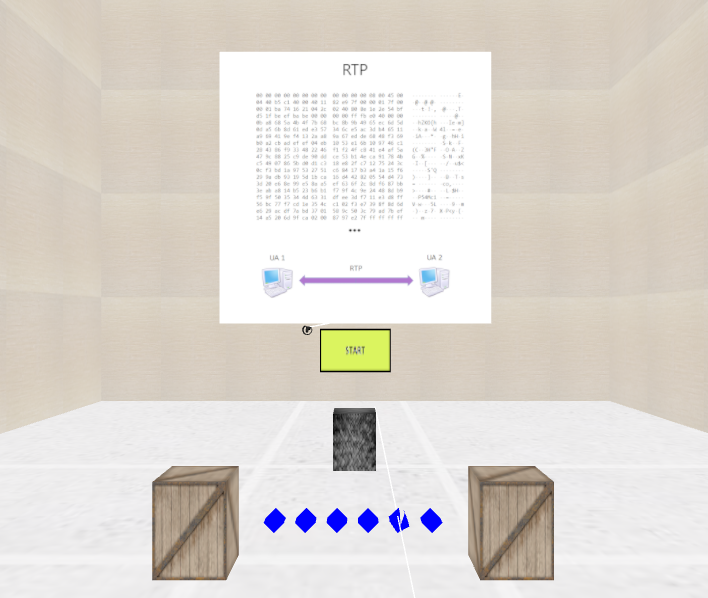
\includegraphics[width=15cm, keepaspectratio]{img/resultados/15-RTP.png}
  \caption{Transmisión de Datos Multimedia a través de Paquetes RTP}
  \label{fig:15-RTP}
\end{figure}

\begin{figure}
  \centering
  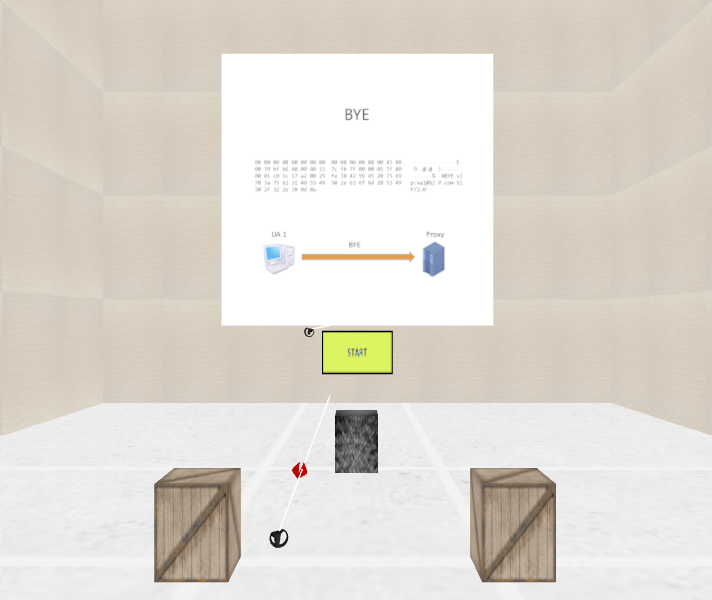
\includegraphics[width=15cm, keepaspectratio]{img/resultados/16-BYE.png}
  \caption{Mensaje BYE Enviado para Terminar la Llamada}
  \label{fig:16-BYE}
\end{figure}

\begin{figure}
  \centering
  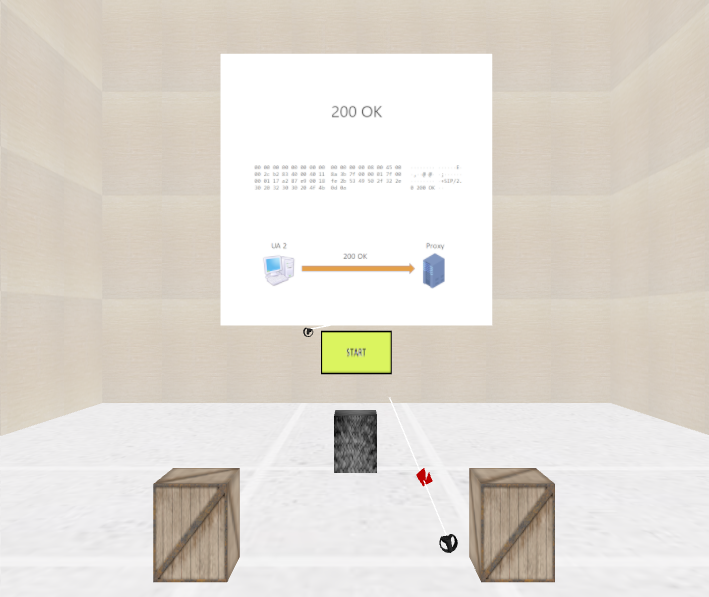
\includegraphics[width=15cm, keepaspectratio]{img/resultados/18-200OK.png}
  \caption{Confirmación del Fin de la Llamada con un 200 OK}
  \label{fig:18-200OK}
\end{figure}



%%%%%%%%%%%%%%%%%%%%%%%%%%%%%%%%%%%%%%%%%%%%%%%%%%%%%%%%%%%%%%%%%%%%%%%%%%%%%%%%
%%%%%%%%%%%%%%%%%%%%%%%%%%%%%%%%%%%%%%%%%%%%%%%%%%%%%%%%%%%%%%%%%%%%%%%%%%%%%%%%
% CONCLUSIONES %
%%%%%%%%%%%%%%%%%%%%%%%%%%%%%%%%%%%%%%%%%%%%%%%%%%%%%%%%%%%%%%%%%%%%%%%%%%%%%%%%

\cleardoublepage
\chapter{Conclusiones}
\label{chap:conclusiones}


\section{Consecución de objetivos}
\label{sec:consecucion-objetivos}

Esta sección es la sección espejo de las dos primeras del capítulo de objetivos, donde se planteaba el objetivo general y se elaboraban los específicos.

Es aquí donde hay que debatir qué se ha conseguido y qué no. 
Cuando algo no se ha conseguido, se ha de justificar, en términos de qué problemas se han encontrado y qué medidas se han tomado para mitigar esos problemas.

Y si has llegado hasta aquí, siempre es bueno pasarle el corrector ortográfico, que las erratas quedan fatal en la memoria final.
Para eso, en Linux tenemos aspell, que se ejecuta de la siguiente manera desde la línea de \emph{shell}:

\begin{verbatim}
  aspell --lang=es_ES -c memoria.tex
\end{verbatim}

\section{Aplicación de lo aprendido}
\label{sec:aplicacion}

Aquí viene lo que has aprendido durante el Grado/Máster y que has aplicado en el TFG/TFM.
Una buena idea es poner las asignaturas más relacionadas y comentar en un párrafo los conocimientos y habilidades puestos en práctica.

\begin{enumerate}
  \item a
  \item b
\end{enumerate}


\section{Lecciones aprendidas}
\label{sec:lecciones_aprendidas}

Aquí viene lo que has aprendido en el Trabajo Fin de Grado/Máster.

\begin{enumerate}
  \item Aquí viene uno.
  \item Aquí viene otro.
\end{enumerate}


\section{Trabajos futuros}
\label{sec:trabajos_futuros}

Ningún proyecto ni software se termina, así que aquí vienen ideas y funcionalidades que estaría bien tener implementadas en el futuro.

Es un apartado que sirve para dar ideas de cara a futuros TFGs/TFMs.


%%%%%%%%%%%%%%%%%%%%%%%%%%%%%%%%%%%%%%%%%%%%%%%%%%%%%%%%%%%%%%%%%%%%%%%%%%%%%%%%
%%%%%%%%%%%%%%%%%%%%%%%%%%%%%%%%%%%%%%%%%%%%%%%%%%%%%%%%%%%%%%%%%%%%%%%%%%%%%%%%
% APÉNDICE(S) %
%%%%%%%%%%%%%%%%%%%%%%%%%%%%%%%%%%%%%%%%%%%%%%%%%%%%%%%%%%%%%%%%%%%%%%%%%%%%%%%%

\cleardoublepage
\appendix
\chapter{Manual de usuario}
\label{app:manual}

Esto es un apéndice.
Si has creado una aplicación, siempre viene bien tener un manual de usuario.
Pues ponlo aquí.

%%%%%%%%%%%%%%%%%%%%%%%%%%%%%%%%%%%%%%%%%%%%%%%%%%%%%%%%%%%%%%%%%%%%%%%%%%%%%%%%
%%%%%%%%%%%%%%%%%%%%%%%%%%%%%%%%%%%%%%%%%%%%%%%%%%%%%%%%%%%%%%%%%%%%%%%%%%%%%%%%
% BIBLIOGRAFIA %
%%%%%%%%%%%%%%%%%%%%%%%%%%%%%%%%%%%%%%%%%%%%%%%%%%%%%%%%%%%%%%%%%%%%%%%%%%%%%%%%

\cleardoublepage

% Las siguientes dos instrucciones es todo lo que necesitas
% para incluir las citas en la memoria
\bibliographystyle{abbrv}
\bibliography{memoria}  % memoria.bib es el nombre del fichero que contiene
% las referencias bibliográficas. Abre ese fichero y mira el formato que tiene,
% que se conoce como BibTeX. Hay muchos sitios que exportan referencias en
% formato BibTeX. Prueba a buscar en http://scholar.google.com por referencias
% y verás que lo puedes hacer de manera sencilla.
% Más información: 
% http://texblog.org/2014/04/22/using-google-scholar-to-download-bibtex-citations/

\end{document}
